\documentclass[a4paper, 12pt]{article}

\usepackage{geometry}
\usepackage{amsmath}
\usepackage{gvv}

\title{Question 1.4.15}
\author{AI25BTECH11040 - Vivaan Parashar}
\date{\today}

\begin{document}

\maketitle

\section{Question: }
The point which divides the line segment joining the points $\vec{P}(7, -6)$ and $\vec{Q}(3, 4)$ in the ratio $1 : 2$ internally lies in which quadrant?

\section{Solution: }
The point $\vec{C}$ that divides points $\vec{P}$ and $\vec{Q}$ in the ratio $l : m$ is
\begin{align}
    \vec{C} = \frac{m\vec{P} + l\vec{Q}}{l+m}\
\end{align}
$\therefore$ The point $\vec{R}$ dividing $\vec{P}$ and $\vec{Q}$ in the ratio $1:2$ is
\begin{align}
    \vec{R} = \frac{2\cdot\vec{P}+1\cdot\vec{Q}}{1+2}\\
    \vec{R} = \myvec{\frac{17}{3} \\ -\frac{8}{3}}
\end{align}
Clearly this point lies in the 4$^\text{th}$ quadrant.

\pagebreak
\section{Plot: }
\begin{figure}[H]
    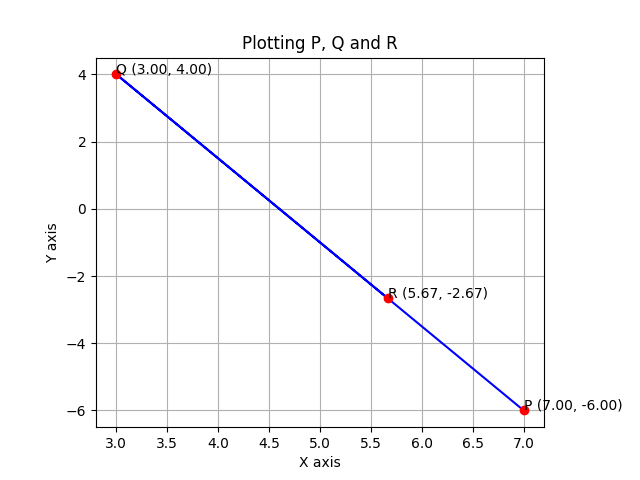
\includegraphics[scale=1]{figs/plot.png}
\end{figure}

\end{document}
